
\documentclass[preprint,3p,twocolumn]{elsarticle}


\usepackage[x11names,dvipsnames,table]{xcolor} %for use in color links
\usepackage[subrefformat=parens,labelformat=parens]{subfig}
\usepackage{svg}
\usepackage{url}
\usepackage{flushend}
\usepackage{xspace}
\usepackage{enumitem}
\usepackage{hyperref}
\usepackage{multirow}
\usepackage{pbox}
\usepackage{pdfcomment}

\definecolor{ao(english)}{rgb}{0.0, 0.5, 0.0}
\newcommand{\todo}[2]{\pdfmargincomment[color=red,author=#1,open=true]{#2}}
\newcommand{\note}[2]{\pdfmargincomment[color=yellow,author=#1,open=true]{#2}}
\newcommand{\closednote}[4]{} % closed notes are hidden. This should obviously be a parameter of \note rather than a separate command.
\newcommand{\answerednote}[4]{\pdfmargincomment[color=green,author=#1-#3,open=true]{#1: #2 \textCR \textCR #3: #4}}
\newcommand{\closedanswerednote}[6]{}


\renewcommand\thesubfigure{\Roman{subfigure}}

\journal{Future Generation Computer Systems}

\begin{document}

\begin{frontmatter}

%% Title, authors and addresses

%% use the tnoteref command within \title for footnotes;
%% use the tnotetext command for theassociated footnotes;
%% use the fnref command within \author or \address for footnotes;
%% use the fntext command for theassociated footnote;
%% use the corref command within \author for corresponding author footnotes;
%% use the cortext command for theassociated footnote;
%% use the ead command for the email address,
%% and the form \ead[url] for the home page:
%% \title{Title\tnoteref{label1}}
%% \tnotetext[label1]{}
%% \author{Name\corref{cor1}\fnref{label2}}
%% \ead{email address}
%% \ead[url]{home page}
%% \fntext[label2]{}
%% \cortext[cor1]{}
%% \address{Address\fnref{label3}}
%% \fntext[label3]{}

\title{Software architectures to integrate workflow engines in science gateways\closednote{Naj}{'what' software architectures? what is their qualifier, adjective?}{Tristan}{There is no qualifier except 'for integrating workflow engines in science gatewats'. They are just software architectures :) The point of the paper is to describe them properly. It's a general formulation to cover any kind of software architecture that is used to integrated workflow engines in science gateways. Does it make sense?}} 

%% use optional labels to link authors explicitly to addresses:
%% \author[label1,label2]{}
%% \address[label1]{}
%% \address[label2]{}

\author[mcgill,creatis]{Tristan Glatard}
\author[mcgill]{Marc-\'Etienne Rousseau}
\author[creatis]{Sorina Camarasu-Pop}

\author[mcgill]{Reza Adalat}
\author[mcgill]{Natacha Beck}
\author[mcgill]{\\Samir Das}
\author[isi]{Rafael Ferreira da Silva}
\author[mcgill]{Najmeh Khalili-Mahani}
\author[criugm]{Pierre-Olivier Quirion}
\author[mcgill]{Pierre Rioux}

\author[criugm]{Pierre Bellec}
\author[mcgill]{Alan C. Evans}

\address[mcgill]{McGill Centre for Integrative Neuroscience, Montreal Neurological Institute, McGill University, Canada.}
\address[creatis]{University of Lyon, CNRS, INSERM, CREATIS, Villeurbanne, France.}
\address[criugm]{Centre de Recherche de l'Institut de G\'eriatrie de Montr\'eal CRIUGM, Montr\'eal, QC, Canada.}
\address[isi]{University of Southern California, Information Sciences Institute, Marina del Rey, CA, USA.}

\begin{abstract}
  We investigate six software architectures commonly used to integrate
  workflow engines in science gateways. In \emph{tight integration},
  the workflow engine shares software components with the science
  gateway. In \emph{service invocation}, the engine is isolated and
  invoked through a specific software interface. In \emph{task
    encapsulation}, the engine is wrapped as a computing task executed
  on the infrastructure. In the \emph{pool model}, the engine is
  bundled in an agent that connects to a central pool to fetch and
  execute workflows. In \emph{nested workflows}, the engine is
  integrated as a child process of another engine. In \emph{workflow
    import}, the engine is integrated through workflow language
  conversion. We describe and evaluate these architectures with
  metrics that measure integration complexity, robustness,
  extensibility, scalability and support for meta-workflows and
  fine-grained debugging\closednote{Naj}{Please be precise, what are
    they?}{Tristan}{Done, thanks}. Results provide insights for
  science gateway architects and workflow engine developers. Tight
  integration and task encapsulation are the easiest to integrate and
  are most robust. Extensibility is equivalent in most
  architectures. The pool model is the most scalable one and
  meta-workflows are only available in nested workflows and workflow
  import. \closednote{Naj}{I find this abstract to be vague, it can be made
    more concise and poignant}{Tristan}{Added a description of the
    architectures, following @pbellec's suggestion.}
\end{abstract}

\begin{keyword}
Workflow engines \sep science gateways \sep software architectures.
\end{keyword}

\end{frontmatter}

%\maketitle

\section{Introduction}

Workflow engines are critical for the efficient and transparent
exploitation of distributed infrastructures in the ecosystem of tools
and services offered by science gateways. Several software
architectures can be adopted to integrate workflow engines in science
gateways, with important consequences on the development effort
required and resulting system.

This paper describes, provides examples and compares such
architectures, based on system-independent representations of their
main components and interactions. It is informed by our experince in
the development and sustained operation of the CBRAIN~\cite{SHER-14}
and VIP~\cite{GLAT-13} science gateways for medical image analysis
during the past 7 years; as well as by lessons learned from several
science gateway and workflow projects such as
SHIWA\footnote{\url{http://www.shiwa-workflow.eu}}.  In this section
we provide background information and definitions of 
workflow engines, science gateways and infrastructures. In
Section~\ref{sec:architectures}, we describe six architectures within
a consistent framework that underlines the functional interactions
between their main software components. In
Section~\ref{sec:evaluation}, the different architectures are
evaluated with metrics measuring integration complexity, robustness,
extensibility, scalability and other specific features. We finally
compare the architectures and highlight recommendations for science
gateway architects and workflow engine developers.

\subsection{Workflow engines}

In the last decade, the e-Science community has developed workflow
systems to help application developers access distributed
infrastructures such as clusters, grids, clouds and web
services. These efforts resulted in tools among which
Askalon~\cite{fahringer2005askalon},
Hyperflow~\cite{balis2016hyperflow}, MOTEUR~\cite{GLAT-08i},
Pegasus~\cite{deelman2005pegasus,Deelman201517},
Swift~\cite{zhao2007swift}, Taverna~\cite{oinn2004taverna},
Triana~\cite{taylor2007triana}, VisTrails~\cite{callahan2006managing}
and WS-PGRADE~\cite{Kacsuk2012}. Such workflow engines usually
describe applications in a high-level language with specific data and
control flow constructs, parallelization operators, visual edition
tools, links with domain-specific application repositories, provenance
recording and other features. An overview of workflow system
capabilities is available in~\cite{deelman2009workflows}.

At the same time, toolboxes have been emerging in various scientific
domains to facilitate the assembly of software components in
consistent ``pipelines''. In neuroimaging, our primary domain of
interest, tools such as Nipype (Neuroimaging in Python, Pipelines and
Interfaces~\cite{gorgolewski2011nipype}), PSOM (Pipeline System for
Octave and Matlab~\cite{bellec2012pipeline}), 
PMP (Poor Man's Pipeline~\cite{Ad-DabbaghY2006}), RPPL~\cite{1174106}, SPM (Statistical
Parametric Mapping~\cite{ashburner2011spm}) and FSL (FMRIB Software
Library~\cite{Jenkinson2012782}) provide abstractions and functions to
handle the data and computing flow between processes implemented in a
variety of programming languages. Such tools were interfaced to
computing infrastructures, in particular
clusters\closednote{Tristan}{Reverted from Marc's 'cluster
  scheduler'}{}{}, to execute tasks at a high throughput. Some of
these tools also support advanced features such as provenance
tracking, \closednote{Naj}{should we not mention PMP which is used for
  CIVET?}{Tristan}{Done, as discussed.} or  redundancy detection across
analyses to avoid re-computation. A wide array of workflows
have been implemented using these pipeline systems and are now shared across
neuroimaging groups world-wide, which represents a tremendous
opportunity for science gateways to leverage. Domain-specific engines
nicely complement e-Science systems that are more oriented towards the
exploitation of distributed computing infrastructures, in particular
grids and clouds.

In this paper, a
\emph{workflow engine} (also abbreviated \emph{engine}) is a piece of
software that submits interdependent computing \emph{tasks} to an
\emph{infrastructure} (local server, cluster, grid or cloud) based on
a workflow description (a.k.a \emph{workflow}), \closednote{Naj}{I think and is redundant here, you can replace is with a comma}{Tristan}{yes!} using input data
that may consist of files, database entries or simple parameter
values. Although simplistic, this definition covers both e-Science workflow systems and
domain-specific pipeline systems.\closednote{Marc-e}{To remain consistent with above descriptions}{Tristan}{yes!} Some workflow engines, usually e-Science
ones, may transfer data across the infrastructure, and others, usually
domain-specific ones, may leave this role to external processes. Workflows
may be expressed in any language, including high-level XML or JSON
dialects such as Scufl or Hyperflow, and low-level scripting languages
such as Bash.

\subsection{Science gateways}

Science gateways are used to share resources within a community and to
provide increased performance and capacity through facilitated access
to storage and computing power. They are often accessible through a
web interface that helps users manage access rights, data transfers,
task execution, and authentication on multiple computing and storage
locations. Workflow engines are part of this ecosystem as core
components to implement and execute
applications. \closednote{Naj}{provide examples?}{Tristan}{Examples
  are mentioned in the last paragraph of this section. Moved it next.}

Various science gateways have been developed, including frameworks
such as Apache Airavata~\cite{marru2011apache}, the Catania Science
Gateway Framework~\cite{ardizzone2012decide} and
WS-PGRADE/gUSE~\cite{Kacsuk2012}. Numerous science gateways were built
using such frameworks~\cite{kacsuk2014science,ardizzone2012decide} or
as standalone systems~\cite{SHER-14,GLAT-13}. Most of these systems
include one or several workflow engines.

% Software properties: integration effort, extensibility, robustness,
% scalability, specific features

Integration between workflow engines and science gateways varies
across systems. Some science gateways are tailored to a particular
engine, while other ones are more general and host applications
executed by different types of engines. %Some gateways may not even use any
%workflow engine and focus on the execution of simple tasks.

Extensibility is an important property of the integration. New
workflows are added frequently, different types and versions of
workflow engines may be integrated over time, and different kinds of
infrastructure can be targeted. 

Scalability is also a crucial concern for such multi-user,
high-throughput systems. For this purpose, science gateways may
balance the load among different instances of the same engine, start
new engines elastically using auto-scaling techniques such as the ones
reviewed in~\cite{lorido2012auto}, and use advanced task scheduling
policies on the infrastructure to improve performance, fault-tolerance
and fairness among users.

Robustness is highly desirable as well since it is key to a
good user experience. Simple architectures facilitate the
implementation effort towards robust interactions which, in turn, have
a positive impact on characteristics such as gateway predictability,
transparency, reliability, traceability and
reproducibility. \closednote{Marc-Etienne}{I find that something is
  weak in this last paragraph. Robustness will help with transparency,
  sure, but it seems only a small facet.  Also, the text seem to
  timidly favor architectures with less components/interactions
  without much explanation... Complex systems can be robust, but at
  greater costs...  Here is one: "Architectures showing reduced system
  complexity will greatly facilitate the implementation effort towards
  robust interactions which, in turn, have a positive impact on
  characteristics such as gateway predictability, transparence,
  general reliability and results traceability and reproducibility;
  characteristics that are also key to a good user
  experience."}{Tristan}{Agreed, fixed as
  suggested.}\closednote{Tristan}{Work on the this sentence again.}{Tristan}{done.}

Other specific features may also be available, for instance
data vizualisation and quality control, workflow edition, debugging
instruments, or social tools among users. \closednote{Naj}{I think using etc after such as, for example and e.g. is not correct. --sorry for being pedantic}{Tristan}{You are completely right, this is now fixed.}

\subsection{Infrastructure}

Infrastructure consists of the computing and storage
resources involved in workflow execution, as well as the software
services used to access these resources. Infrastructure can be
composed of computing or file servers, databases, clusters, grids or
clouds. Some workflow engines and science gateways may require specific
characteristics, such as the presence of a shared file system between
the computing nodes, the availability of a global task meta-scheduler,
the presence of a file catalog, etc. In the analysis presented below,
such specific requirements are not discussed. Instead, we consider the
infrastructure as an abstract system that can execute tasks and store
data regardless of the enabling mechanisms.

\section{Architectures}
\label{sec:architectures}

Architectures to integrate workflow engines in science gateways are
diagrammed in Figure~\ref{fig:architectures} using the graphical
notations shown in
Figure~\ref{fig:notations}. Table~\ref{table:system-classification}
summarizes the classification of a few systems by architecture.

\closednote{Marc-e}{A
  few things bother me a bit with the notation fig., making it harder
  to assimilate 1- The interactions are padded in the middle of other
  stuff (Administrator, Data) 2- The Software component example says
  "Science gateway", should it not be empty?  3- The red arrow to
  explain the use of red; it looks like a very specific type of
  interactions instead of the desired "any interactions or components
  can be red meaning...", especially with 'a' and 'd' which the reader
  does not know the meaning yet.  Maybe a little red arrow and square
  with "Red used when specific to workflow execution"?  I don't have a
  great solution...  Red has special meaning, maybe remove it from the
  other pics (workflow eng, tasks) as it creates lots of visual
  interference when looking for red?  4- Order in text jumps all over
  the fig notations. Explanations are given for, in order: Components,
  workflow engine, interactions, abstract interactions, red color,
  tasks, data (no Administrator?)...  Could re-ordering the fig fix
  this? A figure figure legend could go a long way too (are there some
  in this journal?)  }{Tristan}{Marc-E, is Figure 1 better now?}
\closednote{Naj}{I propose a table of definitions.}{Tristan}{Added
  information in Figure 1 and removed the corresponding text.}


%http://ieeexplore.ieee.org/stamp/stamp.jsp?tp=&arnumber=4782949

\begin{figure}
\centering
\def\svgwidth{0.8\columnwidth}
\input{figures/notations.pdf_tex}
\caption{Graphical notations}
\label{fig:notations}
\end{figure}

\begin{figure*}
\centering
\hspace*{0.2\columnwidth}
\subfloat[Tight integration]{
\def\svgwidth{0.6\columnwidth}
\input{figures/tight.pdf_tex}
\label{archi:tight}
}
\hfill
\subfloat[Service invocation]{
\def\svgwidth{0.6\columnwidth}
\input{figures/service.pdf_tex}
\label{archi:service}
\hspace*{0.2\columnwidth}
}\\
\hspace*{0.2\columnwidth}
\subfloat[Task encapsulation]{
\def\svgwidth{0.6\columnwidth}
\input{figures/sub-task.pdf_tex}
\label{archi:sub-task}
}
\hfill
\subfloat[Pool]{
\def\svgwidth{0.6\columnwidth}
\input{figures/agent.pdf_tex}
\label{archi:agent}
\hspace*{0.2\columnwidth}
}\\
\subfloat[Nested workflows. Left: abstract model. Right: instantiation with service invocation.]{
\def\svgwidth{0.9\columnwidth}
\input{figures/nested-1.pdf_tex}
\def\svgwidth{0.9\columnwidth}
\input{figures/nested-2.pdf_tex}
\label{archi:nested}
}\\
\subfloat[Workflow import. Left: abstract model. Right: instantiation with service invocation.]{
\def\svgwidth{0.5\columnwidth}
\input{figures/import-1.pdf_tex}
\hfill
\def\svgwidth{0.5\columnwidth}
\input{figures/import-2.pdf_tex}
\label{archi:import}
}
\caption{Architectures}
\label{fig:architectures}
\end{figure*}
\begin{table*}
\centering
\footnotesize
\rowcolors{1}{white}{gray!25}
\begin{tabular}{ll}
  \textbf{Architecture} & \textbf{Systems} \\
  \hline
  Tight & \pbox{1.5\columnwidth}{
          Catania Science Gateway Framework~\cite{ardizzone2012decide},
          Distributed application runtime environment (DARE~\cite{maddineni2012distributed}),
          DECIDE~\cite{ardizzone2012decide}$^{c,n}$, LONI Pipeline Environment$^n$~\cite{dinov2009efficient}
          }
  \\
  Service & \pbox{1.5\columnwidth}{
            Apache Airvata~\cite{marru2011apache}, e-BioInfra~\cite{shahand2015data}$^{w,n}$, HubZero with Pegasus~\cite{CPE:CPE3257}, MoSGrid~\cite{kruger2014mosgrid}$^w$, System in~\cite{wu2010accelerating}, Vine Toolkit~\cite{DBLP:journals/scpe/SzejnfeldDKKKKLPTWDNW10}, Virtual Imaging Platform~\cite{GLAT-13}$^n$, WS-PGRADE/gUSE framework~\cite{Kacsuk2012},
            Science gateways in~\cite{kacsuk2014science}$^w$
            } \\
  Task & CBRAIN and PSOM~\cite{GLAT-16}$^n$, CBRAIN and FSL$^n$\\
  Pool & SHIWA pool~\cite{ROGE-13}\\
  Nested & \pbox{1.5\columnwidth}{SHIWA Simulation Platform (Coarse-Grained Interoperability~\cite{terstyanszky2014enabling})$^w$, HubZero with Pegasus (via hierarchical workflows)~\cite{Deelman201517}, Tavaxy~\cite{Abouelhoda2012}.
           }\\
  Import & SHIWA Simulation Platform (Fine-Grained Interoperability)~\cite{plankensteiner-prodan-etal:2013}$^w$, Tavaxy~\cite{Abouelhoda2012}, system in~\cite{delaGarza2016}.
\end{tabular}
\caption{Classification of science gateways based on the architecture used to integrate workflow engines. $^c$: based on the Catania Science Gateway Framework. $^w$: based on WS-PGRADE/gUSE. $^n$: used for neuroimaging.}
\label{table:system-classification}
\end{table*}

\subsection{Interactions}

The interactions involved in the architectures are described below and
labeled as in Figure~\ref{fig:architectures}.

\begin{enumerate}[leftmargin=0cm,itemindent=0.65cm,label=\texttt{(\alph*)}]

\item Workflow integration: consists in adding a new workflow to the
  system so that users can execute it. It is triggered by an
  administrator of the science gateway and it results in an interface,
  for instance a web form, where users can enter the parameters of the
  workflow to be executed. The interaction has two steps:
  (\texttt{a$_1$}) the programs used in the workflow are installed on
  the infrastructure, which may require administrative privileges;
  (\texttt{a$_2$}) the workflow is configured in the science gateway
  so that it becomes available to users. Note that integrating a
  workflow is not the same process as integrating a workflow
  \emph{engine}.
\item Task control: operations to manage tasks on the infrastructure,
  including: authentication, submission, monitoring, termination,
  deletion, etc. Controlling tasks requires to deal with the
  heterogeneous batch managers and meta-schedulers that might be
  available on the infrastructure. When the infrastructure is a grid
  or a cloud, it may for instance be achieved using libraries that
  implement standards such as SAGA (Simple API for Grid
  Applications~\cite{goodale2006saga}), DRMAA (Distributed Resource
  Management Application API~\cite{troger2012distributed}), or OCCI
  (Open Cloud Computing Interface~\cite{edmonds2012toward}).
\item Data control: operations to manage data on the infrastructure,
  such as: upload, download, deletion, browsing, replication, caching,
  etc. Data movements can be triggered by the user in the science
  gateway (\texttt{$c_1$}), to upload input data or download processed
  data. They can also be performed by the workflow engine
  (\texttt{$c_2$}), to transfer workflow data (inputs, outputs, or
  intermediate results) across the infrastructure so that tasks can
  use it. The infrastructure might offer various data storage backends
  with heterogeneous interfaces. \closedanswerednote{Marc-Etienne}{this -c2- can be also trigerred
    by the user}{Tristan}{No, it can't: this is by definition an interaction between the workflow engine and the infrastructure. It is used to transfer data to/from tasks. I reworded a bit, is it clearer now?}
    {Marc-e}{I meant, "using c1", a user in some platforms (CBRAIN), can trigger
    some operations across the infrastructure, as in c2... not just up/download data.
    And I clearly see now that this is in fact the case in III, c is not differentiated. Closing this thread for good.}
  Tools and services such as JSAGA~\cite{reynaud2010uniform} or Data Avenue~\cite{hajnal2014data}
  can be used to homogeneize these interfaces.
\item Workflow control: operations to control workflow execution in an
  engine, including: workflow submission, monitoring, termination,
  etc. Workflow control can be coarse-grained (black box) or
  fine-grained (white box). In a coarse-grained model, the various
  tasks created by a workflow execution are masked and the user only
  has a global view of the workflow execution. In a fine-grained
  model, user is exposed to the workflow topology, i.e. to the outputs
  of the individual tasks, their statuses, dependencies and so on.
\item Sub-task control: operations used by tasks to submit sub-tasks
  on the infrastructure, including: submission, monitoring,
  termination, deletion, etc. Sub-task control is similar to
  interaction \texttt{b}, except that information about the parent
  of a sub-task is usually available and used for
  additional control. For instance, the parent task may wait for all
  its sub-tasks to complete before finishing, and conversely all the
  sub-tasks may be terminated if the parent task is killed.
\item Pool-agent: specific to the pool architecture described in
  Section~\ref{sec:pool}. This is an interaction used when agents
  retrieve work from a central pool. It covers agent registration and
  de-registration to the pool, protocols to send work from the pool to
  the agent, mechanisms to update work status, and so on. A similar
  type of interaction is used in pilot-job
  systems~\cite{turilli2015comprehensive} and other agent-based
  computing models.
\item Workflow conversion: translation from one workflow language to
  another one. This interaction may not be available or implementable
  for every workflow language. It has been developed mostly for
  well-structured and relatively simple workflow languages such as between GWorkflowDL
  and Scufl~\cite{OLAB-09}, and between the 4 languages that were involved in the
  SHIWA initiative.
\end{enumerate}


\subsection{Tight integration}

See Figure~\subref*{archi:tight}. The workflow engine is tightly
integrated with the science gateway, which means that it is deployed
on the same machine and potentially shares code, libraries and other
software components with the science gateway. For instance, the
workflow engine might be a portlet in a Liferay portal or a model
in a Ruby on Rails application. The workflow engine and the science
gateway usually share a database where applications, users and other
resources are stored\closednote{sorina}{VIP and Moteur also share the
  WorkflowsDB}{Tristan}{Yes, you are right. This is an example where
  such abstract architectures may not completely apply in real
  life. See comment about ``blended'' architectures in the
  discussion. In case of VIP, the sharing of the DB is more an
  implementation detail rather than a strong architectural pattern: we
  could avoid sharing the DB if we wanted.}.  In this model, task and
data control are both initiated from the science gateway. Interactions
\texttt{b} and \texttt{c$_2$} are initiated from the workflow engine
while \texttt{c$_1$} comes from other parts of the science gateway,
for instance a data management interface. As in any other model, the
installation of new workflows in the science gateway (\texttt{a$_2$})
and infrastructure (\texttt{a$_1$}) is done by an administrator, for
security reasons. This is the model adopted in the Catania Science
Gateway Framework~\cite{ardizzone2012decide} (see specific documentation on
workflows\footnote{\url{http://bit.ly/1oQrzvQ}}), in the Distributed
application runtime environment
(DARE)~\cite{maddineni2012distributed}, in
Galaxy~\cite{goecks2010galaxy}, and in the LONI Pipeline
Environment~\cite{dinov2009efficient}. Note that tightly integrated
architectures may provide advanced workflow edition features which are
not covered by our analysis.
%The Catania Science Gateway Framework would be a good illustration here (workflow engine is a Java portlet), but I can't find a suitable figure about it.
%CIPRES~\cite{miller2010creating} (on which the Neuroscience gateway
%described in~\cite{sivagnanam2015early} is based) % \note{Tristan}{There is no workflow engine in there.}

\subsection{Service invocation}

\begin{figure*}
\centering
\def\svgwidth{1.5\columnwidth}
\input{figures/VIP.pdf_tex}
\caption{Architecture of the Virtual Imaging Platform (service
  invocation).  Step \texttt{3} corresponds to interaction \texttt{d}
  in Figure~\ref{fig:architectures}(II), step \texttt{2} corresponds to
  interaction \texttt{c$_1$}, step \texttt{4} maps to interaction
  \texttt{b}, and steps 7 and 9 map to \texttt{c$_2$} (in VIP, workflow data transfers are
  performed by the tasks and embedded in their descriptions).}
\label{fig:vip-architecture}
\end{figure*}

See Figure~\subref*{archi:service}. The workflow engine is available
externally to the science gateway, as a service. The science gateway
controls the service through a specific interaction (\texttt{d}) that
might be implemented as a web-service call (e.g., RESTful or SOAP), as
a command-line or as any other method that offers a well-defined
interface to the workflow engine. The workflow engine might be invoked
either as a black box that completely masks the infrastructure and
tasks, or as a white box that allows for some interaction with
them. The workflow engine is responsible for controlling the tasks on
the infrastructure (\texttt{b}) and for performing the required data
transfers to execute them (\texttt{c$_2$}). User data is usually
managed through the science gateway (\texttt{c$_1$}), although it
might as well be delivered by the workflow engine directly to the
user.

This architecture is largely adopted, in systems such as Apache
Airvata~\cite{marru2011apache}, Vine
Toolkit~\cite{DBLP:journals/scpe/SzejnfeldDKKKKLPTWDNW10}, Virtual
Imaging Platform~\cite{GLAT-13}, the system
in~\cite{wu2010accelerating} and the WS-PGRADE/gUSE
framework~\cite{Kacsuk2012}. The integration between the
HubZero science gateway and the Pegasus workflow engine performed
in~\cite{CPE:CPE3257} also uses a service architecture where the
\texttt{d} interaction is implemented as a set of calls to Pegasus'
command-line tools (e.g., pegasus-status, pegasus-plan,
etc.). Figure~\ref{fig:vip-architecture} shows the architecture of the
Virtual Imaging Platform, where the MOTEUR workflow
engine~\cite{GLAT-08i} is invoked through a service.

\subsection{Task encapsulation}
\closednote{Marc-e}{May I propose
  another name here? Either "Task-centric" or "Task Oriented". My
  reasoning is that the WE is just another task, as well as the
  sub-tasks themselves.}{Tristan}{I agree: sub-tasking is not the
  integration model, it is the process that engines use when they
  are integrated as tasks. I think 'task encapsulation' is more
  consistent  with 'service invocation' than 'task-oriented'}

See Figure~\subref*{archi:sub-task}. The workflow engine is wrapped in
a particular task that can submit sub-tasks to the science gateway
through interaction \texttt{e}. The workflow engine keeps track of the
dependencies between the sub-tasks, but their execution is delegated
to the science gateway that executes them on the infrastructure
through interaction \texttt{b}. Although the science gateway has no
global vision of the workflow, it can keep track of the sub-tasks
submitted by a given task, for instance to cancel them when
the task is canceled. The science gateway may also implement
mechanisms to facilitate the handling of task dependencies, for
instance basic dependency lists as available in most cluster managers
(see for instance attribute \texttt{depend} of option \texttt{-W} in
Torque\footnote{\url{http://docs.adaptivecomputing.com}}).

The science gateway also transfers both user and workflow data across
the infrastructure, so that interactions \texttt{c$_1$} and
\texttt{c$_2$} are both covered by \texttt{c}. In practice, both
\texttt{c$_1$} and \texttt{c$_2$} can be implemented using the same
pieces of code.

Task encapsulation is implemented in CBRAIN~\cite{SHER-14} where it is
used to integrate the FSL toolkit~\cite{Jenkinson2012782} and the PSOM
workflow engine~\cite{bellec2012pipeline}. The CBRAIN-FSL integration
allows to leverage FSL pipelines written in low-level workflow
languages (Linux executables and scripts) that submit tasks uniformly
through a specific tool called fsl\_sub. It is diagrammed in
Figure~\subref*{fig:cbrain-fsl-architecture}, where the science gateway is
represented by components \texttt{CBRAIN portal} and \texttt{CBRAIN
  execution server} and the infrastructure consists of \texttt{Storage
  servers} and \texttt{Computing cluster with shared file system}.

The CBRAIN-PSOM integration~\cite{GLAT-16} is shown in
Figure~\subref*{fig:cbrain-psom-architecture}. The PSOM workflow engine
adopts a pilot-job architecture~\cite{turilli2015comprehensive} where
a master coordinates workflow execution by submitting workers and
establishing direct communication channels with them. Note how this
peculiar execution model is well supported by task encapsulation.

\begin{figure*}
\centering
\subfloat[CBRAIN-FSL integration.]{
\def\svgwidth{\columnwidth}
\input{figures/CBRAIN-FSL.pdf_tex}
\label{fig:cbrain-fsl-architecture}
} \hfill \subfloat[CBRAIN-PSOM integration. Figure
reproduced from~\cite{GLAT-16}.]{\def\svgwidth{\columnwidth}
  \input{figures/CBRAIN-PSOM.pdf_tex
}
\label{fig:cbrain-psom-architecture}
}
\caption{CBRAIN architecture for workflow engine integration
  (task encapsulation).  1: User sends data and workflow execution request to
  storage server(s) and CBRAIN portal. 2: CBRAIN portal sends
  execution request to execution server on cluster. 3: Execution
  server transfers data from storage server(s). 4-5: Execution server
  starts workflow engine (FSL tool or PSOM master) via task
  scheduler. 6: Workflow engine submits sub-tasks to execution server
  (FSL tasks or PSOM agents). 7-8: Execution server starts sub-tasks
  through task scheduler (FSL sub-tasks or PSOM workers). FSL sub-tasks will run locally
  instead of being submitted again to CBRAIN through interaction 6. 8':
  (PSOM only) PSOM master and workers execute workflow. 9. Execution
  server transfers results to storage server(s). Interaction
  \texttt{b} in Figure~\ref{fig:architectures}(III) is implemented by steps
  \texttt{4}, \texttt{5}, \texttt{7} and \texttt{8} (regular
  interactions with batch manager). Interaction \texttt{c} is
  implemented by steps \texttt{3} and \texttt{9}. Interaction
  \texttt{e} is implemented by step \texttt{6} (for FSL: through a
  modified version of the fsl\_sub script available in
  \url{https://github.com/aces/cbrain-plugins-neuro}; for PSOM:
  through a specific development in PSOM).}
\label{fig:cbrain-sub-tasking}
\end{figure*}

\subsection{Pool model}
\label{sec:pool}
See Figure~\subref*{archi:agent}. Workflows are submitted by the
science gateway to a central pool through interaction
\texttt{d}. Agents connect to the pool asynchronously to retrieve and
execute workflows through interaction \texttt{f}. Agents may be
started according to various policies, for instance to ensure load
balancing. Workflow engine controls tasks and data on the
infrastructure through interactions \texttt{b} and \texttt{c$_2$},
science gateway transfers user data through interaction
\texttt{c$_1$}, and administrator installs workflows through
interaction \texttt{a$_1$} and \texttt{a$_2$}.

The pool model was implemented in the SHIWA pool~\cite{ROGE-13}
diagrammed in Figure~\ref{fig:shiwa-pool-architecture}, where agents
can wrap different types of workflow engines to execute workflows
expressed with different languages.

\begin{figure*}
\centering
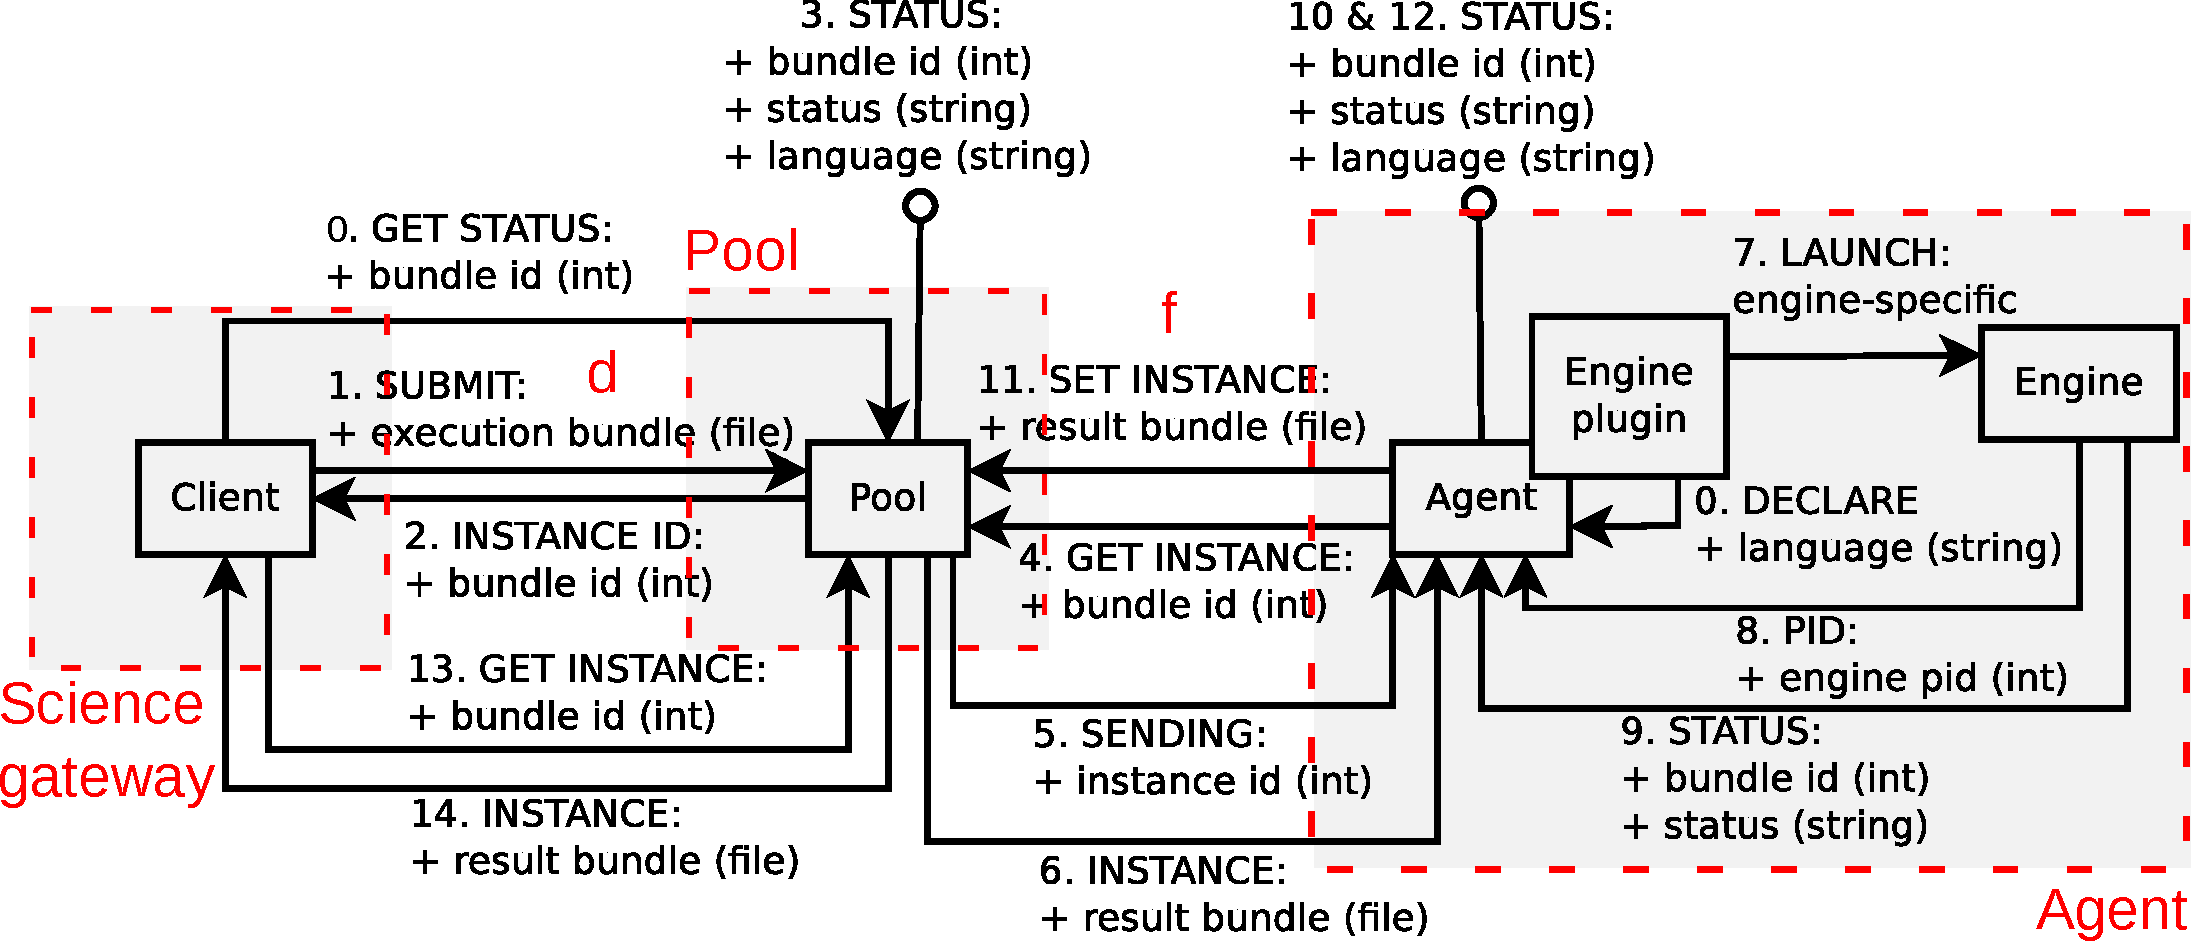
\includegraphics[width=1.5\columnwidth]{figures/pool-interactions.pdf}
\caption{Architecture of the SHIWA pool. Circle-terminated arrows
  indicate messages that are broadcast to all pool
  clients. Interaction \texttt{d} of Figure~\ref{fig:architectures}(IV) is
  implemented by 3 different calls to the pool: workflow
  submission (\texttt{1} \& \texttt{2}), workflow status retrieval
  (\texttt{0} \& \texttt{3})\closednote{sorina}{I suppose letters come
    here from the initial pool-model figure; it's a bit puzzling when
    mixed with letters from Fig 2}{Tristan}{Fixed.}, and workflow
  retrieval (\texttt{13} \& \texttt{14}). \closednote{Marc-e}{Maybe
    easier to follow if the following would be in fig legend instead
    of here, as for 2 previous figures}{Tristan}{fixed} Interaction
  \texttt{f} is implemented through 2 types of calls: workflow
  instance retrieval (\texttt{4}, \texttt{5} and \texttt{6}), and
  workflow instance update (\texttt{11} and \texttt{12}). Workflow
  instance retrieval is used by the agents to fetch work from the
  pool. Workflow instance update is used by the agents to update
  workflow statuses.  Calls \texttt{0}, \texttt{7}, \texttt{8} and
  \texttt{9} are used by
  workflow engine plugins to declare their supported language and to
  launch engines, and by workflow engines to report their status to
  the agent. These calls are specific to the SHIWA Pool implementation
  of the \texttt{agent} component and therefore have no corresponding
  representation in Figure~\ref{fig:architectures}(IV). Figure reproduced
  from~\cite{ROGE-13}.}
\label{fig:shiwa-pool-architecture}
\end{figure*}


\subsection{Nested workflows}

See Figure~\subref*{archi:nested}. In nested workflows
(Figure~\subref*{archi:nested}-Left), workflows include other
workflows that are executed by a \emph{child} engine. Parent
and child engines might use different languages and might run on
different infrastructures. A parent workflow is
also called meta-workflow. The science gateway communicates with the
parent engine through abstract interaction \texttt{*$_1$}. The science
gateway also communicates with the infrastructure to transfer user
data through abstract interactions \texttt{*$_2$} and
\texttt{*$_3$}. Both workflow engines communicate with the
infrastructure through abstract interactions \texttt{*$_4$} and
\texttt{*$_5$}. The parent engine communicates with the child engine
through abstract interaction \texttt{*$_6$}. Administrator installs
workflows through interactions \texttt{a$_1$} and \texttt{a$_2$}.

Nested workflows are abstract architectural patterns that can be
instantiated in the various architectures described previously. We
focus on instantiation with the service invocation model
(Figure~\subref*{archi:nested}-Right) as this is the most used
architecture. In the instantiation, we assume that the parent and
child workflow engines are distinct pieces of software that require
different workflow services invoked by distinct \texttt{d}
interactions. If this is not the case then workflow services can be
collapsed in a single one with a \texttt{d} interaction with
itself. An example of such interaction is the use of hierarchical
workflows in Pegasus~\cite{Deelman201517}.
Workflow engines communicate with infrastructures using
\texttt{b} and \texttt{c$_2$}. Science gateway transfers user data to
infrastructures using \texttt{c$_1$} interactions.


Nested workflows have long been available in workflow engines, for
instance in the Taverna workbench~\cite{oinn2004taverna}. They are
also used implicitly in several platforms where workflow engines are
wrapped in workflow tasks as any other command-line tool. Nested
workflows were notably used by the SHIWA Science Gateway to implement
so-called Coarse-Grained workflow
interoperability~\cite{terstyanszky2014enabling}, i.e. to integrate
various workflow engines in a consistent
platform. Figure~\ref{fig:shiwa-architecture} shows the architecture
used in the SHIWA Simulation Platform for nested workflow execution
with service invocation.
\begin{figure*}
\centering
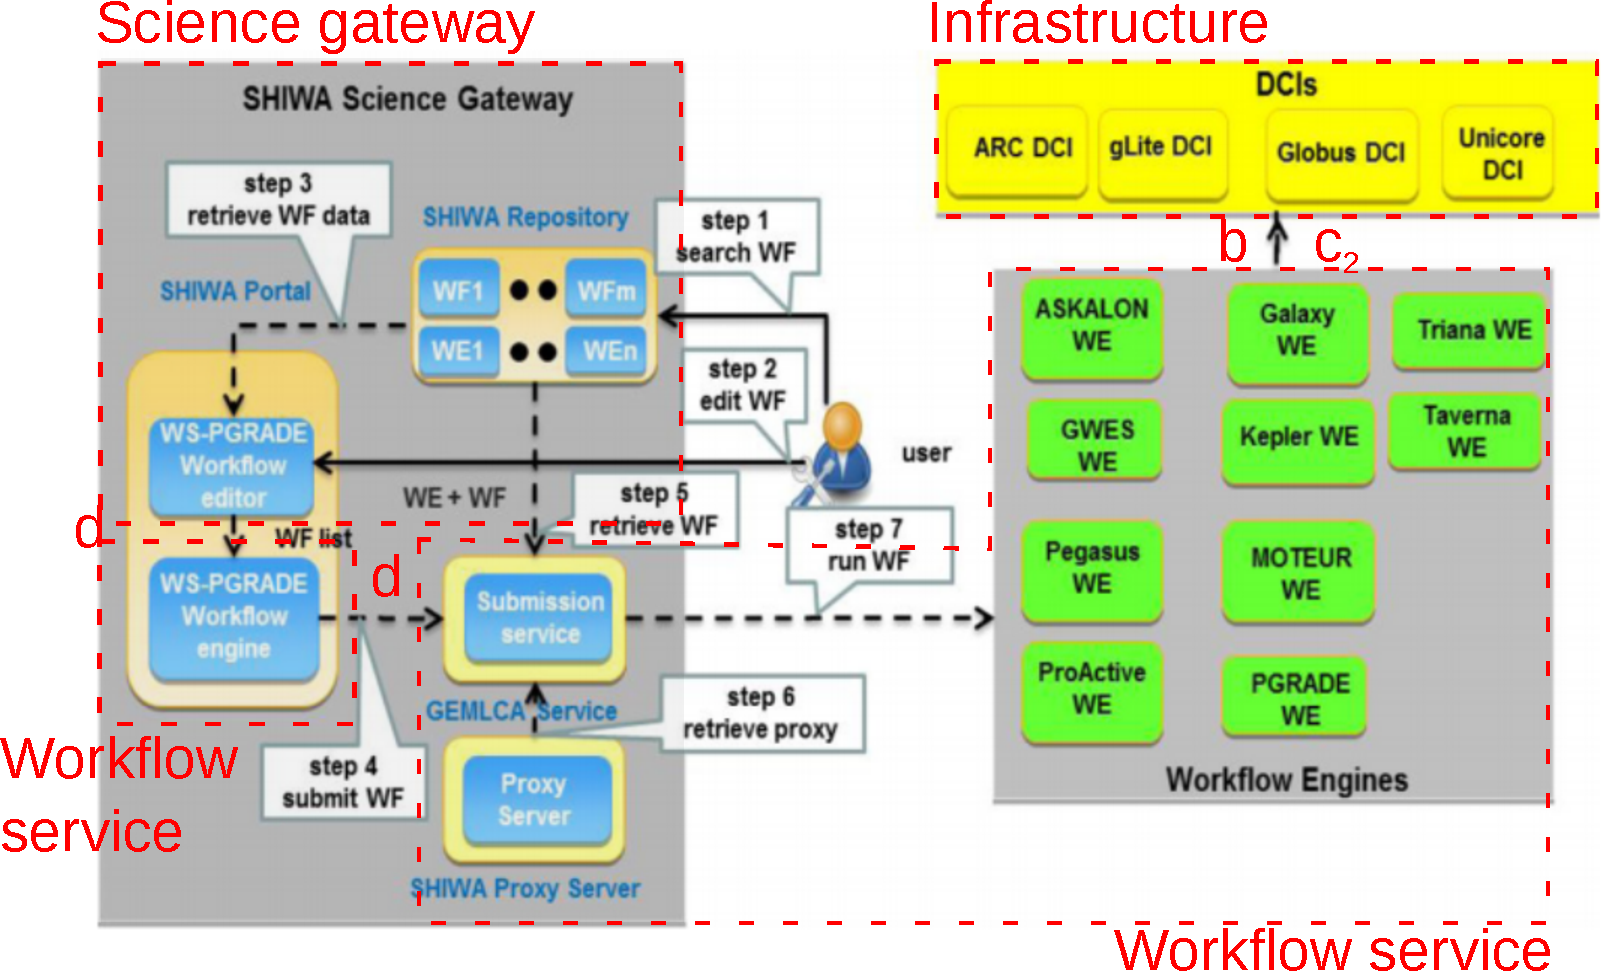
\includegraphics[width=1.5\columnwidth]{figures/shiwa-science-gateway.pdf}
\caption{Nested workflow execution through SHIWA Science Gateway. The
  parent workflow engine is \texttt{WS-PGRADE}, invoked as a service
  in the Science Gateway (step \texttt{1}, interaction \texttt{d} on
  Figure~\ref{fig:architectures}(V)-Right). Ten different child engines can be used by nested
  workflows, invoked through the \texttt{Submission service} (step
  \texttt{2}, interaction \texttt{d}). Each of these engines can
  submit tasks and transfer data to a distributed computing
  infrastructure (\texttt{DCI}, step \texttt{3}, interactions
  \texttt{b} and \texttt{c$_2$}). User data interactions (\texttt{c$_1$}) and
  application porting ones (\texttt{a}) are not represented. Figure
  reproduced from~\cite{terstyanszky2014enabling} with permission of
  the first author.}
\label{fig:shiwa-architecture}
\end{figure*}

\subsection{Workflow import}

See Figure~\subref*{archi:import}. This is an abstract model
instantiated with the service invocation architecture for
consistency. Workflows are integrated in the science gateway through
format conversion from a native format to the science gateway
format. Workflow import is usually an offline process that is not
involved in workflow execution. A few systems have implemented
workflow import. In the SHIWA Simulation Platform, it is implemented
through the IWIR language that provides a common language for
portability across grid workflow
systems~\cite{plankensteiner-prodan-etal:2013} and allows to convert
among $n$ workflow languages using $2n$ interactions instead of $n^2$.
Tavaxy~\cite{Abouelhoda2012}
allows to import, merge and run Taverna~\cite{oinn2004taverna} and
Galaxy~\cite{goecks2010galaxy} workflows; when some workflow parts
cannot be imported, workflows are run by Tavaxy as nested workflows
using their native engine. The work in~\cite{delaGarza2016} describes
workflow import from KNIME~\cite{Berthold2008} to WS-PGRADE/gUSE and
from Galaxy~\cite{goecks2010galaxy} to WS-PGRADE/gUSE.
\closednote{Tristan}{Add description of a real system}{Tristan}{Would
  require to reproduce a figure from another paper. The concept seems
  simple enough to not require a figure.}

%Furthermore, both systems provide web-portals allowing users to share and publish their workflows: These are the myExperiment portal for Taverna [23, 24] and the Public Pages for Galaxy [13].

\section{Evaluation}

\label{sec:evaluation}

The architectures described in Section~\ref{sec:architectures} are
evaluated in Table~\ref{table:evaluation} using 5 main criteria:
integration complexity, robustness, extensibility, scalability and
other specific features. Criteria break down to specific metrics where
\emph{lower value indicates better performance}. For each criterion, a
global score is computed by summing up the individual metrics. We
ensure that the different metrics in a criterion measure similar
entities so that they can be summed. The criteria and metrics are
explained hereafter.


\begin{table*}
\footnotesize
\centering
\begin{tabular}{rcccccc}
                                     & \textbf{Tight}
                                     & \textbf{Service}
                                     & \textbf{Task}
                                     & \textbf{Pool}
                                     & \textbf{Nested}
                                     & \textbf{Import} \\
\cellcolor[HTML]{EEEEEE}\textbf{Integration complexity}& \multicolumn{6}{l}{\cellcolor[HTML]{EEEEEE}}\\
  Total components -- \texttt{I$_1$} & \cellcolor[HTML]{99FF99}2
                                     & \cellcolor[HTML]{99DD99}3
                                     & \cellcolor[HTML]{99FF99}2
                                     & \cellcolor[HTML]{99BB99}4
                                     & \cellcolor[HTML]{999999}5
                                     & \cellcolor[HTML]{99DD99}3\\
Total interactions -- \texttt{I$_2$} & \cellcolor[HTML]{99FF99}5
                                     & \cellcolor[HTML]{99EE99}6
                                     & \cellcolor[HTML]{99FF99}5
                                     & \cellcolor[HTML]{99DD99}7
                                     & \cellcolor[HTML]{999999}11
                                     & \cellcolor[HTML]{99DD99}7\\
\textbf{Total} (total software pieces) & \cellcolor[HTML]{99FF99}\textbf{7}
                                     & \cellcolor[HTML]{99E899}\textbf{9}
                                     & \cellcolor[HTML]{99FF99}\textbf{7}
                                     & \cellcolor[HTML]{99D299}\textbf{11}
                                     & \cellcolor[HTML]{999999}\textbf{16}
                                     & \cellcolor[HTML]{99DD99}\textbf{10}\\
\cellcolor[HTML]{EEEEEE}\textbf{Robustness}& \multicolumn{6}{l}{\cellcolor[HTML]{EEEEEE}}\\
Specific components -- \texttt{R$_1$} & \cellcolor[HTML]{99FF99}0
                                     & \cellcolor[HTML]{99CC99}1
                                     & \cellcolor[HTML]{99FF99}0
                                     & \cellcolor[HTML]{999999}2
                                     & \cellcolor[HTML]{999999}2
                                     & \cellcolor[HTML]{99CC99}1\\
  Specific interactions -- \texttt{R$_2$} & \cellcolor[HTML]{99EB99}2
                                     & \cellcolor[HTML]{99D699}3
                                     & \cellcolor[HTML]{99FF99}1
                                     & \cellcolor[HTML]{99C299}4
                                     & \cellcolor[HTML]{999999}6
                                     & \cellcolor[HTML]{99D699}3\\
  \textbf{Total} (execution software pieces)& \cellcolor[HTML]{99F099}\textbf{2}
                                     & \cellcolor[HTML]{99D399}\textbf{4}
                                     & \cellcolor[HTML]{99FF99}\textbf{1}
                                     & \cellcolor[HTML]{99B699}\textbf{6}
                                     & \cellcolor[HTML]{999999}\textbf{8}
                                     & \cellcolor[HTML]{99D399}\textbf{4}\\
\cellcolor[HTML]{EEEEEE}\textbf{Extensibility}& \multicolumn{6}{l}{\cellcolor[HTML]{EEEEEE}}\\
  New engine type -- \texttt{E$_1$}  & \cellcolor[HTML]{99C599}3
                                     & \cellcolor[HTML]{99A899}4
                                     & \cellcolor[HTML]{99E299}2
                                     & \cellcolor[HTML]{99C599}3
                                     & \cellcolor[HTML]{999999}4.5
                                     & \cellcolor[HTML]{99FF99}1\\
New engine version -- \texttt{E$_2$} & \cellcolor[HTML]{999999}1
                                     & \cellcolor[HTML]{99FF99}0
                                     & \cellcolor[HTML]{999999}1
                                     & \cellcolor[HTML]{99FF99}0
                                     & \cellcolor[HTML]{99FF99}0
                                     & \cellcolor[HTML]{999999}1\\
  New workflow -- \texttt{E$_3$} & \cellcolor[HTML]{99FF99}2
                                     & \cellcolor[HTML]{99FF99}2
                                     & \cellcolor[HTML]{99FF99}2
                                     & \cellcolor[HTML]{99FF99}2
                                     & \cellcolor[HTML]{99FF99}2
                                     & \cellcolor[HTML]{999999}3\\
New infrastructure -- \texttt{E$_4$} & \cellcolor[HTML]{99DD99}4
                                     & \cellcolor[HTML]{99DD99}4
                                     & \cellcolor[HTML]{99FF99}3
                                     & \cellcolor[HTML]{99DD99}4
                                     & \cellcolor[HTML]{999999}6
                                     & \cellcolor[HTML]{99DD99}4\\
  \textbf{Total} (difficulty to extend) & \cellcolor[HTML]{99D299}\textbf{10}
                                     & \cellcolor[HTML]{99D299}\textbf{10}
                                     & \cellcolor[HTML]{99FF99}\textbf{8}
                                     & \cellcolor[HTML]{99E899}\textbf{9}
                                     & \cellcolor[HTML]{999999}\textbf{12.5}
                                     & \cellcolor[HTML]{99E899}\textbf{9}\\
\cellcolor[HTML]{EEEEEE}\textbf{Scalability}& \multicolumn{6}{l}{\cellcolor[HTML]{EEEEEE}}\\
Multiple engine instances -- \texttt{S$_1$}& \cellcolor[HTML]{999999}2
                                     & \cellcolor[HTML]{99CC99}1
                                     & \cellcolor[HTML]{99FF99}0
                                     & \cellcolor[HTML]{99FF99}0
                                     & \cellcolor[HTML]{99CC99}1
                                     & \cellcolor[HTML]{99CC99}1\\
Distributed engines -- \texttt{S$_2$}& \cellcolor[HTML]{999999}1
                                     & \cellcolor[HTML]{999999}1
                                     & \cellcolor[HTML]{999999}1
                                     & \cellcolor[HTML]{999999}1
                                     & \cellcolor[HTML]{99FF99}0
                                     & \cellcolor[HTML]{999999}1\\
Task scheduling -- \texttt{S$_3$}    & \cellcolor[HTML]{99FF99}0
                                     & \cellcolor[HTML]{99FF99}0
                                     & \cellcolor[HTML]{999999}1
                                     & \cellcolor[HTML]{99FF99}0
                                     & \cellcolor[HTML]{999999}1
                                     & \cellcolor[HTML]{99FF99}0\\
\textbf{Total} (scalability issues)  & \cellcolor[HTML]{999999}\textbf{3}
                                     & \cellcolor[HTML]{99CC99}\textbf{2}
                                     & \cellcolor[HTML]{99CC99}\textbf{2}
                                     & \cellcolor[HTML]{99FF99}\textbf{1}
                                     & \cellcolor[HTML]{99CC99}\textbf{2}
                                     & \cellcolor[HTML]{99CC99}\textbf{2}\\
\cellcolor[HTML]{EEEEEE}\textbf{Specific features}& \multicolumn{6}{l}{\cellcolor[HTML]{EEEEEE}}\\
  Meta-workflow  -- \texttt{O$_1$}    & \cellcolor[HTML]{999999}1
                                     & \cellcolor[HTML]{999999}1
                                     & \cellcolor[HTML]{999999}1
                                     & \cellcolor[HTML]{999999}1
                                     & \cellcolor[HTML]{99FF99}0
                                     & \cellcolor[HTML]{99FF99}0\\
  Fine-grained debugging -- \texttt{O$_2$}   & \cellcolor[HTML]{99FF99}0
                                     & \cellcolor[HTML]{99FF99}0
                                     & \cellcolor[HTML]{999999}1
                                     & \cellcolor[HTML]{99FF99}0
                                     & \cellcolor[HTML]{999999}1
                                     & \cellcolor[HTML]{99FF99}0\\
  \textbf{Total} (missing features) & \cellcolor[HTML]{99CC99}\textbf{1}
                                     & \cellcolor[HTML]{99CC99}\textbf{1}
                                     & \cellcolor[HTML]{999999}\textbf{2}
                                     & \cellcolor[HTML]{99CC99}\textbf{1}
                                     & \cellcolor[HTML]{99CC99}\textbf{1}
                                     & \cellcolor[HTML]{99FF99}\textbf{0}\\
\end{tabular}

\caption{Architecture evaluation. Lower values (brighter colors) indicate better performance. Cell color is set as follows: (1) on each row, metric values are
  normalized between 0 (best value) and 1 (worst value):
  $m'=\frac{m-m_{\mathrm{min}}}{m_{\mathrm{max}}-m_{\mathrm{min}}}$ where
  $m$ is the metric value, $m_{\mathrm{min}}$ and $m_{\mathrm{max}}$
  are the minimal and maximal values among all architectures; (2) the RGB hexadecimal color code of the cell
  is \texttt{\#99XX99}, where X=\texttt{round}(F-6m') (\texttt{round} rounds a number to the nearest integer). \closednote{Tristan}{Use 6. Round to the nearest integer.}{Tristan}{Fixed.}}
\label{table:evaluation}
\end{table*}

\subsection{Evaluation metrics}

\emph{Integration complexity} is obtained by counting the total number of
interactions and components on the architecture diagram. It breaks
down to the following 2 metrics:
\begin{itemize}[leftmargin=0cm,itemindent=0.35cm,itemsep=0cm]
\item Total number of components (\texttt{I$_1$}), and
\item Total number of interactions (\texttt{I$_2$}).
\end{itemize}
One may wonder whether infrastructure should be counted in
\texttt{I$_1$} since it is usually not developed by the groups who
integrate workflow engines in science gateway. However, integrating an
infrastructure in the architecture usually requires some technical
effort (e.g., account creation, software installation, APIs, etc.), which is
why we keep it in the metric. The two metrics are summed to obtain a
global score that measures the
total number of software pieces to develop, including interactions and
components. 

\emph{Robustness of workflow execution} measures the likelihood that
workflow execution fails due to errors in the components or with the
interactions in the software architecture. Errors coming
from the infrastructure (e.g., unavailable data or terminated tasks)
or workflows (e.g., wrong user input or application errors) are not
covered since they do not stem directly from the software
architecture. Robustness is measured here as a consequence of global
complexity since complex architectures tend to be more prone to
failure. More precisely, robustness is determined as the number of
software components and interactions that are specific to workflow
execution:
\begin{itemize}[leftmargin=0cm,itemindent=0.35cm,itemsep=0cm]
\item Components (\texttt{R$_1$}): number of specific components
  involved in workflow executions. Science
gateway, for instance, is \emph{not} specific to workflow execution
since it is used to authenticate users, add new workflows, transfer
user data, etc.
\item Interactions (\texttt{R$_2$}): number of specific interactions
  involved in workflow executions.
\end{itemize}
These specific components and interactions are the ones represented in
red in the architecture diagrams in
Figure~\ref{fig:architectures}. \texttt{R$_1$} and \texttt{R$_2$} are
summed to obtain the global score for this criterion, which measures
the total number of software pieces that are specifically involved in
the workflow execution.

\emph{Extensibility} measures the difficulty to replace or add
elements in the architecture. It is determined as the number of interactions and
components that need to be modified when a new element is
added. Modification of a component is required when its code needs to
be updated or recompiled (science gateway or workflow service), or
when a new piece of software has to be installed (infrastructure
only). Modification of an interaction is deemed necessary when the
parameters involved in this interaction are modified.  Extensibility
breaks down to 4 metrics depending on the type of element that has to
be added or replaced:
\begin{itemize}[leftmargin=0cm,itemindent=0.35cm,itemsep=0cm]
\item New engine type (\texttt{E$_1$}): number of interactions or
  components to modify to integrate a new type of workflow engine in
  the architecture. Workflow engines belong to different types when
  they cannot be invoked using the same interface. 
\item New engine version (\texttt{E$_2$}): number of interactions or
  components to modify to integrate a new version of a workflow engine
  in the architecture, assuming that another version of the same
  engine type is already available. Different versions of a workflow
  engine share the same interface, i.e. they can be invoked using the
  same software. When this is not the case, the different versions are
  considered as different engine types. Components are not treated
  equally regarding engine version updates. Components whose only
  function is to host the workflow engine, i.e. workflow services and
  agents, are not counted in E$_2$ because updates in such components
  are assumed to be straightforward. On the contrary, modifications of
  components that have other functions than wrapping the engine,
  i.e. science gateway and infrastructure, are counted in E$_2$
  because updates in these components require more effort, e.g. new
  release of the science gateway, gaining administrative privileges on
  the infrastructure, etc.
\item New workflow (\texttt{E$_3$}): adding a new workflow is a very
  common operation that does not require modifying software components
  or interactions. We measure the difficulty to integrate a new
  workflow by counting the number of interactions required
  to integrate a new workflow in the architecture, assuming
  that the engine type and version required to execute this workflow
  are already available.
\item New infrastructure (\texttt{E$_4$}): number of interactions or
  components to modify to integrate a new type of infrastructure in
  the architecture. Adding a new infrastructure allows to provide more
  computing or storage power, to access specific types of resources
  (e.g., GPUs, clouds), or to enforce execution policies (e.g.,
  constrain data to remain in a particular network domain).
%\item New science gateway: \todo{Not sure if this makes sense}.
\end{itemize}
The 4 metrics are summed to obtain a global index that measures the
difficulty to extend the architecture. \closednote{Naj}{I would rather compare each metric separately, this woudl also give a sense of how different architectures compare across metrics}{Tristan}{Metrics are compared separately too, see Table 2 and discussion.} Note that some extensions may
involve several metrics in practice. For instance, adding a new type
of engine may help integrate new infrastructures when interactions
\texttt{b} and \texttt{c$_2$} are already present for the new engine
and infrastructure.  \closednote{Rafael}{Adding a new engine type may
  also allow run in different infrastructures. Maybe it is worth to
  put a sentence to clarify that the metric account for it
  separately.}{Tristan}{It will not *allow* because interaction c1
  would still need to be developed. But it will definitely facilitate
  it. I added a note on this after the description of the metrics.}


\emph{Scalability} corresponds to the ability of the architecture to
cope with high workloads. It is measured by counting the potential
scalability issues in the architectures, i.e. the missing scalability
features. Features are evaluated using a 3-level metric: 0 means that
the feature is very easy to enable, 1 means that it can be implemented
but with some difficulty, and 2 means that the feature cannot
realistically be implemented. \closednote{Naj}{how do you metricize
  "nonesensical amount fo effors?"}{Tristan}{You don't :) Rephrased to
  'cannot realistically be implemented'. At some point it's a matter
  of common sense and experience to draw the line between what is
  easily implemented and what is more tricky. I would like to avoid
  'impossible' because nothing is impossible to implement if enough
  effort is put.} Four different features are identified:
\begin{itemize}[leftmargin=0cm,itemindent=0.35cm,itemsep=0cm]
\item Multiple engine instances (\texttt{S$_1$}): possibility to have
  more than 1 engine instance in the architecture. Workflow engines
  may require important amounts of resources when several workflows,
  or large workflows, are executed. At some point, it may be required
  for the science gateway to distribute the load among several
  engines. \texttt{S$_1$}=0 when adding a new engine instance is a
  fully automated process, i.e. the workflow engine only has to be
  started. In this case, elastic engines are possible, i.e. some kind
  of auto-scaling mechanism can be implemented to control the number
  of engine instances in the architecture. \texttt{S$_1$}=1 when
  adding a new engine instance requires some form of manual
  intervention (e.g., two-factor authentication), which prevents easy
  implementations of elastic engines. \texttt{S$_1$}=2 when new engine
  instances cannot be added.
\item Distributed engines (\texttt{S$_2$}): possibility to distribute
  the execution \emph{of a single workflow} among different engine
  instances. In our scope, this feature focuses on the capabilities of
  the architecture rather than these of the workflow
  engine. \texttt{S$_2$}=0 when distributed engines are possible in
  the architecture, \texttt{S$_2$}=1 when they require specific
  developments in the workflow engine.  \closednote{Rafael}{$S_2$
    would be 2 if the paradigm does not allow to distribute the
    orchestration? e.g., workflow executions implemented within MPI
    jobs, in Pegasus PMC and dispel4Py.}{Tristan}{The problem is that
    it is very difficult to define ``does not allow to''. For
    instance, why couldn't you hack Pegasus PMC so much that it
    becomes possible to distribute workflow executions in several MPI
    jobs coordinated by an MPI job? Moreover, S2=2 is not used so I'd
    prefer to leave it like this, unless you have a suggestion to
    reflect this in the text.}
\item Task scheduling (\texttt{S$_3$}): task scheduling is a difficult
  issue that depends more on the implementation of specific algorithms
  in the science gateway, workflow engine and infrastructure than on
  the architecture used to integrate the workflow engine in the
  science gateway. Some architectures, however, complicate the task
  scheduling problem by introducing additional software layers or
  creating tasks with specific characteristics. \texttt{S$_3$}=0 when
  the architecture does not introduce any additional complexity to the
  scheduling problem, and \texttt{S$_3$}=1 otherwise.
\end{itemize}
The 3 metrics are summed to obtain a global measure of the scalability
issues that are present in the architecture.

\emph{Specific features} include:
\begin{itemize}[leftmargin=0cm,itemindent=0.35cm,itemsep=0cm]
\item Meta-workflow (\texttt{O$_1$}): ability to describe
  meta-workflows from existing workflows. Meta-workflows offer an
  additional level of flexibility to build workflows from reusable
  components. \texttt{O$_1$}=0 when the feature is available,
  \texttt{O$_1$}=1 otherwise.
\item Fine-grained debugging (\texttt{O$_2$}): availability of
  fine-grained debugging information about workflow tasks (white-box
  workflow).  Fine-grained information about workflow tasks is
  required to properly troubleshoot workflow executions.
  \texttt{O$_2$}=0 when such information is easy to access,
  \texttt{O$_2$}=1 otherwise.
\end{itemize}
\texttt{O$_1$} and \texttt{O$_2$} are summed to obtain a total number of missing specific
features in the architecture.

%"A Formal Approach to Support Interoperability in Scientific
%Meta-workflows" (reviewed for IWSG and JoGC) has a formal model to
%evaluate CGI and FGI.
%"four major approaches for workflow interoperability include a,b,c,d" (see Terstyanzky et al, "Enabli%ng scientific workflow sharing through CGI...", FGCS 2014) -> read this ref.
% http://www.oreilly.com/programming/free/files/software-architecture-patterns.pdf

The architectures described in Figure~\ref{fig:architectures} are
evaluated along these metrics in the remainder of this Section.

\subsection{Tight integration}

\paragraph{Integration complexity} This architecture does not require any
component in addition to the science gateway and infrastructure
(\texttt{I$_1$=2}). It involves 5 interactions: \texttt{a$_1$},
\texttt{a$_2$}, \texttt{b}, \texttt{c$_1$} and \texttt{c$_2$}
(\texttt{I$_2$=5}).

\paragraph{Robustness} No component is specific to workflow execution
(\texttt{R$_1$}=0), but interactions \texttt{b} and \texttt{c$_2$} are
(\texttt{R$_2$}=2).

\paragraph{Extensibility} Integrating a new type of workflow engine
requires to modify the science gateway as well as interactions
\texttt{b} and \texttt{c$_2$} (\texttt{E$_1$}=3). Updating a workflow
engine version requires modifications in the science gateway
(\texttt{E$_2$}=1).  Inserting a new workflow is done through
interactions \texttt{a$_1$} and \texttt{a$_2$}
(\texttt{E$_3$}=2). Adding a new infrastructure generates updates in
interactions \texttt{a$_1$}, \texttt{b}, \texttt{c$_1$} and
\texttt{c$_2$} (\texttt{E$_4$}=4).

\paragraph{Scalability} Adding a new engine instance requires a new
instance of the science gateway, which is in general not possible
(\texttt{S$_1$}=2). Specific IT setups such as load-balancing between
web server instances might be used to deal with this
issue. \closedanswerednote{Tristan}{What-about load-balancing between web
  server instances?}{Marc-e}{Would that really be considered a real
  architectural feature or an IT hack?}{Tristan}{I agree, we should
  keep IT setups out of the picture. Depending on the internals of the
  science gateway, such hacks may or may not be feasible. I added a
  sentence to mention this possibility, without changing the score.}
Distributed engines are not available by default
(\texttt{S$_2$}=1). The scheduling of tasks on the infrastructure is
as complex as in any other architecture since the workflow engine
might implement any kind of scheduling policy (\texttt{S$_3$}=0).

\paragraph{Specific features} Meta-workflows are not supported by default
(\texttt{O$_1$}=1).  Debugging is not an issue since the science
gateway can retrieve any information from the workflow engine directly
(\texttt{O$_2$}=0).

\subsection{Service invocation}

\paragraph{Integration complexity} Service invocation requires a workflow service
in addition to the science gateway and infrastructure
(\texttt{I$_1$}=3). The architecture involves 6 interactions:
\texttt{a$_1$}, \texttt{a$_2$}, \texttt{b}, \texttt{c$_1$},
\texttt{c$_2$} and \texttt{d} (\texttt{I$_2$}=6).

\paragraph{Robustness} The workflow service is a component specific to
workflow execution (\texttt{R$_1$}=1). Workflow execution also
involves 3 specific interactions: \texttt{b},
\texttt{c$_2$} and \texttt{d} (\texttt{R$_2$}=3).

\paragraph{Extensibility} Adding a new type of workflow engine
requires to implement the corresponding workflow service, to modify
interaction \texttt{d}, and to implement interactions \texttt{b} and
\texttt{$c_2$} (\texttt{E$_1$}=4). New engine versions can be added by
updating the workflow service without modifying any interaction or
component (\texttt{E$_2$}=0). Updating the engine version in a
workflow service does not count in \texttt{E$_2$} since the only goal of this component
is to wrap the engine.  New workflows are added in the science gateway
or in the workflow engine through interactions \texttt{a$_1$} and
\texttt{a$_2$} (\texttt{E$_3$}=2). Adding a new type of infrastructure
requires updates in interactions \texttt{a$_1$}, \texttt{b},
\texttt{$c_1$} and \texttt{$c_2$} (\texttt{E$_4$}=4).

\paragraph{Scalability} The service architecture supports multiple
engine instances through multiple workflow services. In VIP for
instance, this feature has been available from release 1.17. A basic
load-balancing mechanism is available that sends new workflow
executions to the engine instance which has the least active
executions. To avoid ``black-hole'' syndromes created by failing
engine instances, engine instances are automatically disabled when
workflows cannot be submitted to them. Adding a new engine instance,
however, requires manual intervention to declare the new instance in
the science gateway (\texttt{S$_1$}=1). Consequently, elastic engines
are difficult to implement because they require a mechanism to update
the science gateway configuration when a new engine instance is
available. Distributing the execution of a single workflow in multiple
engines is usually not possible unless the workflow engine has
specific abilities (\texttt{S$_2$}=1). The scheduling of tasks on the
infrastructure is as complex as in any other architecture since the
workflow engine might implement any kind of scheduling policy
(\texttt{S$_3$}=0).

\paragraph{Specific features} Meta-workflows are not supported by default
(\texttt{O$_1$}=1). Fine-grained debugging information is usually easy
to obtain since the workflow service provides direct access to the
engine (\texttt{O$_2$}=0).

\subsection{Task encapsulation}

\paragraph{Integration complexity} Task encapsulation requires only 2
components (\texttt{I$_1$}=2).  It involves 5 interactions:
\texttt{a$_1$}, \texttt{a$_2$}, \texttt{b}, \texttt{c} and
\texttt{e} (\texttt{I$_2$}=5).

\paragraph{Robustness} No component is specific to workflow execution
(\texttt{R$_1$}=0), and only interaction \texttt{e} is
(\texttt{R$_2$}=1)\closedanswerednote{sorina}{I understand why this is 1
  (and why interactions c and b are not counted here), but I wonder
  whether we can simply ignore these interactions because they are not
  specific to workflow execution. As far as robustness is concerned,
  the transfers have to be successful anyway...}{Tristan}{We cannot
  just ignore these interactions in the architecture because they are
  required for the system to work. The transfers have to be successful
  but data movements in the workflow will use the same code as data
  movements done in the science gateway, which will make this
  architecture more robust than service for instance. In VIP, for
  instance, the code used in the GASW wrapper to transfer data (c2) is
  completely independent from the ``file transfer'' module in the
  platform (c1), which is detrimental to robustness}{Tristan}{Closed,
  see github issue \#7.}.

\paragraph{Extensibility} Integrating a new type of workflow engine
requires to develop interaction \texttt{e} and to install the engine
on the infrastructure (\texttt{E$_1$}=2). Updating an engine version
in the architecture shares the same mechanism as version updates of
other tasks, which requires an update on the
infrastructure (\texttt{E$_2$}=1).  New workflows are integrated by
creating a new task in the science gateway through interactions
\texttt{a$_1$} and \texttt{a$_2$} (\texttt{E$_3$}=2). Adding a new
infrastructure requires to update interactions \texttt{a$_1$},
\texttt{b} and \texttt{c} in the science gateway (\texttt{E$_4$}=3).

%\todo{Integrating a workflow engine as a sub-task
%only requires to implement interaction \texttt{e} (\texttt{I$_2$}=1)
%and to install the workflow engine on the infrastructure
%(\texttt{I$_3$}=1). A new task type is created in the science gateway
%only when a new workflow has to be integrated (see M$_4$), but this is
%not required to integrate the engine itself (\texttt{I$_1$}=0).}

\paragraph{Scalability}
New engine instances are spawned and executed on the infrastructure as
any other task upon user submission (\texttt{S$_1$}=0). This is a
major interest of task encapsulation. Distributed engines are not
supported by default (\texttt{S$_2$}=1). Task scheduling is slightly
more complex than in the other approaches due to the special role of
the task that executes the workflow engine (\texttt{S$_3$}=1). Indeed,
the reliability of this task is critical since all the sub-tasks in
the workflow depend on it and, depending on the recovery capabilities
of the workflow engine, may need to be resubmitted if the workflow
task fails. The workflow task is also longer than all its sub-tasks,
which increases its chances of failure. In addition, task parameters,
for instance estimated walltime, are more difficult to estimate for
the workflow task than for the sub-tasks because workflows are by
definition more complex than their sub-tasks: errors on sub-task
parameter estimations accumulate in the workflow, and additional
control constructs such as tests and loops may further increase the
uncertainty. Such parameter estimation errors may generate issues such
as selection of wrong batch queues on clusters or task termination due
to exceeded quotas. \closednote{Naj}{The lay reader wonders why?  an
  example like the one offered for interdependencies can
  help}{Tristan}{Done, thanks.} Finally, the interdependencies between
the workflow task and its sub-tasks may create deadlocks when there is
contention. For instance, if only 1 computing resource is available
for the science gateway and if the workflow task is running on it and
submits sub-tasks, then the sub-tasks could only execute when the
resource is available, which will never happen because the workflow
task will not complete until the sub-tasks complete. This
configuration can be generalized to an infrastructure with $n$
resources where $n$ workflows are submitted. In practice, however, the
number of submitted workflows usually remains lower than the number of
computing resources available on this infrastructure, which makes such
deadlocks unlikely to happen. \closednote{Naj}{so is this the solution to
  fixing the above mentioned limitations with
  scalability?}{Tristan}{Unfortunately this is not a solution. We just
  say that this situation is unlikely to happen which is true.}

\paragraph{Specific features} Meta-workflows are not available
(\texttt{O$_1$}=1).  Obtaining fine-grained information about workflow
tasks is not straightforward since the science gateway has no
knowledge about the workflow topology, and the workflow engine is
integrated as a task (\texttt{O$_2$}=1).

\subsection{Pool model}

\paragraph{Integration complexity} The pool model requires a workflow pool and an
agent in addition to the science gateway and infrastructure
(\texttt{I$_1$=4}). It involves 7 interactions: \texttt{a$_1$},
\texttt{a$_2$}, \texttt{b}, \texttt{c$_1$}, \texttt{c$_2$}, \texttt{d}
and \texttt{f} (\texttt{I$_2$}=7).

\paragraph{Robustness} The workflow pool and agent are specific to
workflow execution (\texttt{R$_1$=2}). Interactions \texttt{b},
\texttt{c$_2$}, \texttt{d} and \texttt{f} also are (\texttt{R$_2$=4}).

\paragraph{Extensibility} Adding a new engine type requires to wrap
the engine in the agent and to update interactions \texttt{b} and
\texttt{c$_2$} (\texttt{E$_1$=3}). Updating the version of an engine
is transparent (\texttt{E$_2$=0}) since it only requires updating the
agent that is a component dedicated to the engine. Integrating a new workflow is
done through interactions \texttt{a$_1$} and \texttt{a$_2$}
(\texttt{E$_3$=2}). Integrating a new infrastructure requires updates
in interactions \texttt{a$_1$}, \texttt{b}, \texttt{c$_1$} and \texttt{c$_2$}
(\texttt{E$_4$=4}).

\paragraph{Scalability} New engine instances only require new agents,
which is easily automated (\texttt{S$_1$=0}) and by design very
suitable for elastic computing.\closednote{Naj}{I feel the concept of elastic computing should be mentioned in introductory sections}{Tristan}{You are right, this is now fixed.} For instance, auto-scaling rules can
be implemented to start new agents when the workload in the science
gateway exceeds a certain threshold~\cite{lorido2012auto}. Distributed
engines are not available by default (\texttt{S$_2$=1}) and task
scheduling is as complex as in any other architecture
(\texttt{S$_3$=0}).

\paragraph{Specific features} Meta-workflows are not available by default
(\texttt{O$_1$=1}).  Accessing debugging information is not likely to
be an issue since the workflow pool could implement specific functions
for that (\texttt{O$_2$=0}).

\subsection{Nested workflows with service invocation}

\paragraph{Integration complexity} Setting up a nested workflow
architecture with service invocation requires a science gateway, 2
workflow services and 2 infrastructures (\texttt{I$_1$=5}). The
architecture involves 11 interactions (\texttt{I$_2$=11}):
\texttt{a$_1$} (twice), \texttt{a$_2$}, \texttt{b} (twice), \texttt{c$_1$} (twice),
\texttt{c$_2$} (twice) and
\texttt{d} (twice).
\closedanswerednote{Rafael}{I like the idea of what has been discussed in
  the `integration effort', however I think the name may lead to
  misinterpretations. For example, according to Table 2, it requires
  more effort to integrate in a Tight architecture than in a
  service-based architecture. Considering the principles of software
  engineer, it is simpler to integrate/maintain a system using
  decoupled services. Maybe it should be renamed to something related
  to 'dependencies'.}{Tristan}{In our scope I'm not sure that it's
  simpler to integrate a service architecture than a tightly
  integrated one. But I take your point. 'Dependencies' is not very
  suitable either. What about 'development effort'?}{Tristan}{Replaced
  'Integration effort' with 'global complexity', as discussed in
  github issue \#8.} 

\paragraph{Robustness} The two workflow services are specific to
workflow execution (\texttt{R$_1$=2}). Interactions \texttt{b}
(twice), \texttt{c$_2$} (twice) and \texttt{d} (twice) also
are (\texttt{R$_2$=6}).
\closednote{Marc-e}{I understand both points. However, complexity is
  addressed in Robustness as well... I liked the idea of development effort. It's a tough call.}{Tristan}{Maybe 'integration challenge' is a good compromise.}

\paragraph{Extensibility} Adding a new type of \emph{parent} engine
requires to implement the corresponding service, to implement
interactions \texttt{b} and \texttt{c$_2$} in the parent engine, and
to implement interaction \texttt{d} in the science gateway and in the
parent service (\texttt{E$_1$=5}). Adding a new type of \emph{child}
engine only requires to implement the corresponding service, to
develop interactions \texttt{b} and \texttt{c$_2$} in the child
engine, and to implement interaction \texttt{d} in the parent service
(\texttt{E$_1$=4}). We use \texttt{E$_1$=4.5} in
Table~\ref{table:evaluation} to reflect both conditions. Adding a new
version in the parent or child engine only requires modifying this
engine (\texttt{E$_2$=0}). Adding a new workflow is done through
interaction \texttt{a$_1$} and \texttt{a$_2$}
(\texttt{E$_3$=2}). Adding a new infrastructure requires to
re-implement interactions \texttt{a$_1$}, \texttt{b} and
\texttt{c$_2$} twice, and interaction \texttt{c$_1$} once so that it
can be supported by both workflow engines (\texttt{E$_4$=6}).

\paragraph{Scalability} As in the service architecture, adding a new
workflow instance requires manual configuration in the science gateway
(instance of a parent engine), or in the parent engine (instance of a
child engine) (\texttt{S$_1$=1}). Similarly, elastic engines are
difficult to achieve. Distributed engines are
possible, through meta-workflows (\texttt{S$_2$=0}). Task scheduling
is more complex than in other architectures though, due to the fact
that workflow execution is split in different engines (\texttt{S$_3$=1}).

\paragraph{Specific features}
Meta-workflows are possible, which is one of the main interest of this
architecture (\texttt{O$_1$=0}).  Debugging is difficult because the
science gateway cannot directly access fine-grained information in the
sub-workflow (\texttt{O$_2$=1}).

\subsection{Workflow import with service invocation}

\paragraph{Integration complexity} Workflow import with service invocation
requires the same components as for service invocation
(\texttt{I$_1$}=3). It requires an additional \texttt{g} interaction
for workflow import (\texttt{I$_1$}=7).

\paragraph{Robustness} Since workflow conversion is not involved in
the execution (it is an offline process), metrics are as in the
service architecture (\texttt{R$_1$=1}, \texttt{R$_2$=3}).

\paragraph{Extensibility} Since adding a new type of workflow engine
aims at supporting more workflows, we consider that it only requires
to re-implement interaction \texttt{g} in this architecture  (\texttt{E$_1$=1}). Note,
however, that implementing interaction \texttt{g} can require very
substantial work depending on the complexity of the language used by
the new engine. Similarly, adding a
new engine version only requires modifying interaction \texttt{g}
(\texttt{E$_2$=1}).  Adding a new workflow is done through
interactions \texttt{a$_1$}, \texttt{a$_2$} and \texttt{g} (\texttt{E$_3$=3}). As in the
service architecture, interfacing with a new infrastructure requires
modifications in interactions \texttt{a$_1$}, \texttt{b}, \texttt{c$_1$}
and \texttt{c$_2$} (\texttt{E$_4$=4}).

\paragraph{Scalability}  Since workflow conversion is not involved in
the execution (it is an offline process), metrics are as in the
service architecture (\texttt{S$_1$=1},
\texttt{S$_2$=1}, \texttt{S$_3$=0}).

\paragraph{Specific features} Meta-workflows are available after import,
by connecting workflows in the language used in the science gateway
(\texttt{O$_1$=0}). Debugging information is accessible as in the
service invocation architecture (\texttt{O$_2$=0}).

\section{Discussion}

\subsection{Comparison between architectures}

Tight integration and task encapsulation are the simplest
architectures to integrate, followed by service integration, workflow import (with
service invocation) and pool. Nested workflows (with service
invocation) require more integration than the other
architectures. Robustness roughly leads to the same ordering of
architectures, with tight integration and task encapsulation in the top
group, service integration and workflow import (with service
invocation) close behind, pool in a third group, and nested workflows
(with service invocation) at the end. This ordering is consistent
across metrics; it reflects the global complexity of the
architectures.

Regarding extensibility, most architectures are overall comparable,
except nested workflows (with service invocation) which are
significantly behind. This is explained by the complexity of the
nested workflow architecture, with 2 infrastructures and 2 workflow
services. Task encapsulation and workflow import (with service
invocation) perform slightly better when integrating new engines
(\texttt{E$_1$}), which makes them useful architectures for science
gateways that do not focus on a particular engine.\closednote{Naj}{what is
  interesting?}{Tristan}{Rephrased, thanks.}  However, task encapsulation, workflow import (with
service invocation) and tight integration perform worse than the
others when adding engine versions (\texttt{E$_2$}), due to the need
to update infrastructure (task encapsulation), science gateway (tight
integration), or workflow converter (workflow import). Workflow import
performs worse than the others when integrating new workflows
(\texttt{E$_3$}) because of the language conversion step. All
architectures except nested workflows are equivalent when integrating
new infrastructures (\texttt{E$_4$}).

The pool architecture is overall the most scalable, which is not
surprising since it is designed precisely for scalability. Tight
integration is the least scalable and all the other architectures
perform the same overall. The global scalability score, however,
should not conceal \closednote{Naj}{what do you mean by
  mask?}{Tristan}{I guess 'hide' or 'conceal' are better
  words. Fixed.} the unique characteristics of architectures regarding
this criterion. Nested workflows are the only architecture that can
easily accommodate distributed workflow execution, which can be
critical in some cases. At the same time, the scheduling constraints
created by task encapsulation and nested workflows may become problematic \closednote{Naj}{please don't use these from-film-marketing
  words?! :-) }{Tristan}{OK!} depending on the type of targeted
infrastructure. Non-reliable infrastructures\closednote{Naj}{you mean by
  the showstoppers, i.e. the nested workflows which can accommodate
  distributed executions but are limited by scheduling constraints?}{Tristan}{Yes. I rephrased a bit this part.},
for example, could hardly cope with workflow engines being wrapped in
computing tasks as done in task encapsulation. The availability of
multiple engine instances could also become a critical feature for
science gateways with important workloads, which would favor task
encapsulation and pool. \note{Naj}{I feel this paragraph is a bit
  vague, and doesn't distill and contextualize the thorough work
  described before.}

Differences in other specific features should not be neglected. Nested
workflows (with service invocation) and workflow import (with service
invocation) are the only architectures that support meta-workflows;
task encapsulation and nested workflows may complexify
fine-grained debugging. \closednote{Rafael}{I would suggest to provide
  some more examples when this could be interesting.}{Tristan}{Done.}
The availability of fine-grained debugging information may also be
critical to efficient user support.

Table~\ref{table:overall} provides an overall comparison between
architectures, based on the metrics in Table~\ref{table:evaluation}.
Note that this analysis is only for illustration purposes since it
assumes that all criteria have equal weights while real systems would
favor some of them. Overall, task encapsulation, and workflow import (with
service invocation) perform a bit better than tight integration,
service invocation and pool. Nested workflows stands a bit behind for
the reasons mentioned previously.\closednote{Rafael}{I would emphasize
  that this analysis is only for illustration purposes, since it does
  not account for different weights in metrics.}{Tristan}{Done.}
\begin{table*}
\footnotesize
\centering
\begin{tabular}{rcccccc}
                                    & \textbf{Tight}
                                    & \textbf{Service}
                                    & \textbf{Task}
                                    & \textbf{Pool}
                                    & \textbf{Nested}
                                    & \textbf{Import} \\
  Integration (global score)    &
                                    \cellcolor[HTML]{99FF99}{0.00}
                                    & \cellcolor[HTML]{99E899}{0.22}
                                    & \cellcolor[HTML]{99FF99}{0.00}
                                    & \cellcolor[HTML]{99D299}{0.44}
                                    & \cellcolor[HTML]{999999}{1.00}
                                      & \cellcolor[HTML]{99DD99}{0.33}\\
Robustness (global score) &
                                \cellcolor[HTML]{99F099}{0.14}
                                    & \cellcolor[HTML]{99D399}{0.43}
                                    & \cellcolor[HTML]{99FF99}{0.00}
                                    & \cellcolor[HTML]{99B699}{0.71}
                                    & \cellcolor[HTML]{999999}{1.00}
                                    & \cellcolor[HTML]{99D399}{0.43}\\
  Extensibility (global score)  & \cellcolor[HTML]{99D299}{0.44}
                                     & \cellcolor[HTML]{99D299}{0.44}
                                     & \cellcolor[HTML]{99FF99}{0.00}
                                     & \cellcolor[HTML]{99E899}{0.22}
                                     & \cellcolor[HTML]{999999}{1.00}
                                     & \cellcolor[HTML]{99E899}{0.22}\\
Scalability (global score)  & \cellcolor[HTML]{999999}{1.00}
                                     & \cellcolor[HTML]{99CC99}{0.50}
                                     & \cellcolor[HTML]{99CC99}{0.50}
                                     & \cellcolor[HTML]{99FF99}{0.00}
                                     & \cellcolor[HTML]{99CC99}{0.50}
                                     & \cellcolor[HTML]{99CC99}{0.50}\\
Specific features (global score) & \cellcolor[HTML]{99CC99}{0.50}
                                     & \cellcolor[HTML]{99CC99}{0.50}
                                     & \cellcolor[HTML]{999999}{1.00}
                                     & \cellcolor[HTML]{99CC99}{0.50}
                                     & \cellcolor[HTML]{99CC99}{0.50}
                                     & \cellcolor[HTML]{99FF99}{0.00}\\
                                    & \cellcolor[HTML]{99E799}\textbf{2.1}
                                    & \cellcolor[HTML]{99E699}\textbf{2.1}
                                    & \cellcolor[HTML]{99FE99}\textbf{1.5}
                                    & \cellcolor[HTML]{99EF99}\textbf{1.9}
                                    & \cellcolor[HTML]{999999}\textbf{4.0}
                                    & \cellcolor[HTML]{99FF99}\textbf{1.5}\\
\end{tabular}
\caption{Overall evaluation. Brighter colors and lower scores indicate better performance. Scores
  are obtained by summing the normalized global scores ($m'$ values) of
  each criterion in Table~\ref{table:evaluation} and the colors are obtained as in Table~\ref{table:evaluation}. }
\label{table:overall}
\end{table*}

\subsection{Limitations}


A few limitations should be considered when using the results of our
evaluation. First, our evaluation methods aimed to provide comparative
metrics, however the high-level of abstraction used to derive these
metrics hinders the complexity of real systems to some
extent.\closednote{Naj}{Here, you were bashing your article harshly,
  so I rewrote it}{Tristan}{yup, thanks!}. In particular, the
presented architectures are abstract patterns that may be mixed
together in actual systems.\answerednote{Naj}{something about "theoretical
  pattern", and "blending" is jarring, are these common words in the
  computer sci context?}{Tristan}{Better now?} The distinction between tight integration and
service invocation, for instance, may not always be that clear in
practice. Service invocation may also be combined with task
encapsulation in some cases. However, the criteria discussed in this
work would still apply to broadly compare and categorize such cases of
hybrid architectures.

Moreover, all the interactions involved in the architectures were
treated equally while some of them are obviously more complex than
others. For example, interaction \texttt{g} (workflow language
conversion) is clearly more complex than interaction \texttt{d}
(service invocation), and may create much more reliability issues as
well. However, without entering into the details of a particular
system, quantification of the robustness or the amount of development
associated with each interaction and software component will not be
precise.

The particular case of interaction \texttt{g} (workflow language
conversion) requires particular attention when implementing a real
system \closednote{Naj}{so are you discussing it here, or in the
  future?}{Tristan}{It's out of scope, a complete paper in itself. Rephrased this part.} since this interaction may not be easily generalized to any
workflow language. For instance, converting FSL, PSOM or Nipype
pipelines to any other workflow language is problematic because these
engines rely on general-purpose programming languages such as Bash,
Octave and Python, which are much richer than scientific workflow
languages.

The abstract nested workflows and workflow import patterns were
instantiated with service invocation so that they can be analyzed in
the same framework as the other architectures. Other types of
instantiation, for instance nested workflows with task encapsulation,
could also be envisaged. We chose to limit ourselves to instantiations
with service invocation because the resulting architectures are
implemented in real systems, and because service invocation is largely
used. Nevertheless, it could be interesting to explore other types of
instantiations, in particular nested workflows with task
encapsulation.\answerednote{Naj}{I think in the discussion, you may want to close the circle on a statement in introduction, which referred to your 7-year experience with CBRAIN and VIP}{Tristan}{Good idea, will think about it.}

The particular technical or historical context of a science gateway
project may obviously influence the choice of an architecture to
integrate workflow engines. For instance, some workflow engines may be
already available as web services\note{Naj}{This is a good place to offer some examples}, which would tend to favor service
invocation, and other science gateways may have strongly tested task
and data control features (interactions \texttt{b} and \texttt{c}),
which would favor task encapsulation. Similarly, adding a new type of engine
may facilitate integration of a new infrastructure when interactions
\texttt{b} and \texttt{c$_2$} are already available. The migration
cost between architectures has been ignored as well.

Finally, workflow engines are only one of the many aspects involved in
the design of a science gateway. Other properties definitely influence
the design of a software architecture, for instance collaborative
features, data visualization, search, authentication, accounting and
so on.

\section{Conclusion}

% Summary of contributions
We have systematically reviewed architectures used to integrate workflow engines in
science gateways. These architectures are described in a system-independent framework
suitable for comparison, illustrated on real systems, and evaluated using novel quantitative metrics that allow simple comparison across architectures. We have discussed the
pros and cons of all the presented architectures based on these metrics.
\closedanswerednote{Rafael}{One thing that is missing in the
  conclusion or the limitations section is to state that this work
  does not intend to quantify the amount of work required to develop
  science gateways using a specific architecture, but the goal is to
  highlight what are the main components and interactions for each
  architecture, and the main advantages and drawbacks. This should
  also be stated in the introduction.}{Tristan}{This is in
  contradiction with the metric on 'integration effort'. What do you
  think?}{Tristan}{Fixed, as discussed in github \#8.}

% Impact of the work
To the best of our knowledge, our work is the first to systematically
review and compare software architectures used to integrate workflow
engines in science gateways.\closednote{Naj}{instead of its kind,
  explain what kind it is, e.g. systematic review of all
  ...}{Tristan}{Done.} So far, the literature on science gateways and
workflow engines has focused on the description of particular systems,
or on the presentation of a particular architecture.  Instead, our
analysis abstracts and evaluates architectural patterns independently
from any particular system. It provides general insight to integrate
science gateways and workflow engines, which we hope will be useful
for software architects.

% Literature on SG architecture Very few works go beyond the
% description of architectures of particular systems. For instance, the work
%in~\cite{Gannon2005} discusses service-oriented architectures for
% science gateways with workflow engines.  The work in
% http://link.springer.com/chapter/10.1007/11596141_3 discusses
% service-oriented architectures for science gateways, with a workflow
% engine. The work in
% http://docs.lib.purdue.edu/cgi/viewcontent.cgi?article=1414&context=nanopub
% highlights 4 TeraGrid science gateways (GridChem, LEAD, nanoHUB,
% CABIG). Architectures are described but there is no real focus on
% workflow engines. GridChem doesn't include any workflow engine,
% which btw make it relevant for integration via sub-tasking. LEAD has
% a workflow engine.

\section{Acknowledgments}

This work is in the scope of the LABEX PRIMES (ANR-11- LABX-0063) of
Universit\'e de Lyon, within the program ``Investissements d’Avenir''
(ANR-11-IDEX-0007) operated by the French National Research Agency
(ANR). This work also falls into the scope of the scientific topics of
the French National Grid Institute (IdG). We thank the site
administrators of the European Grid Initiative and the GGUS support
for their help related to the VIP platform. The CBRAIN team is grateful for the
computing cycles, storage, and support obtained from Compute Canada
(\url{https://computecanada.ca}) and platform development program from CANARIE
 (\url{http://www.canarie.ca/}). The integration between PSOM and CBRAIN was supported by a Brain 
Canada Platform Support Grant, as well as the Canadian Consortium on
Neurodegeneration in Aging (CCNA), through a grant from the Canadian Institute
of Health Research and funding from several partners. This work has been made possible with the support of the Irving Ludmer Family Foundation and
the Ludmer Centre for Neuroinformatics and Mental Health. \closedanswerednote{Marc-e}{Would it be proper to thank EGI?
  Compute Canada? CANARIE?}{Tristan}{Added EGI and Compute Canada. Not sure if
  Canarie should be added. What about Calcul QC?}{Marc-e}{CQ, no. CANARIE, I'd
  say yes since they funded a major chunk of CBRAIN's development.}

\section*{References}

\enlargethispage{5mm}
\bibliographystyle{plain}
\bibliography{biblio}

\end{document}
\endinput
